\documentclass[journal]{IEEEtran}

\usepackage[T1]{fontenc}
\usepackage{amsmath,amsfonts}
\usepackage{newtxtext}
\usepackage{newtxmath}

\usepackage{algorithmic}

\usepackage{cite}
\usepackage{graphicx}
\usepackage{booktabs}
\usepackage{tabularx}
\usepackage{geometry}

\usepackage{tikz}
\usetikzlibrary{positioning, arrows.meta}

\usepackage[hidelinks]{hyperref}

\begin{document}

\title{title}

\author{Andy Babcock \\
    \textit{Steve Sanghi College of Engineering, Northern Arizona University} \\
    Flagstaff, AZ, USA \\
    aab726@nau.edu
}

\maketitle

% ========================================
% 1. lit review & questions and hypotheses
% ========================================

\section{Introduction}
Anxiety and anxiety disorders are one of the most prevalent mental health conditions, predominately affecting youth and young adults, ages 10-24~\cite{BieFengsai2024Rgbo}. In the past 35 years, anxiety disorders have increased by 52\% among adolescents and young adults. Daily anxiety affects nearly all parts of life, especially test-taking in college-age students. Existing anxiety conditions can be heightened during test-taking through stressors such as GPA-based scholarships or working a part-time job. Luckily, anxiety can be mitigated even without changing the specific circumstances that cause it. One way is playing white noise: a 2025 study examined how the anxiety levels of college students undergoing Cognitive Behavioral Therapy (CBT) were changed by white noise~\cite{LiLi2025EoWN}. This study focuses on the difference in anxiety, depression, and sleep quality when only undergoing CBT, and while also listening to white noise in therapy. CBT represents a different dynamic to test-taking, but shares some qualities, such as therapy being an innate stessor, which can compound with external stressors (i.e.: needing to set boundaries with family). Anxiety levels in test-taking can be be monitored for changes from external factors like white noise or music using an Electroencephalogram (EEG) to measure changes in brain activity which is correlated to anxiety.

\section{The Effect of White Noise on Anxiety}
A 2022 paper examines the effect of white noise on anxiety in operating room staff~\cite{ShahrokhiShabnam2022Teow}. Operating rooms share many similarities with test-taking, presenting both inherent stressors (successfully operating on another human) and external stressors (an expectation for the staff to do their jobs well and quickly). Anxiety reduces performance at work, so any simple solution that could potentially decrease anxiety would represent a painless way to improve performance. Noise is an inherent source of anxiety, which disproportionately affects operating rooms more than other medical environments thanks to numerous pieces of loud equipment. Therefore any distraction from that noise could reduce anxiety as well. Previous studies found that music significantly reduces stress, but also reduces the surgeon's auditory processing~\cite[p.~2]{WayT.JustinMD2013EoNo}. A potential middle ground that addresses this issue are less audible, muffled sounds that draw less attention than music would. Thus, the study chose white noise from a suction machine, which is already commonly used in operating rooms.

The paper tests this hypothesis with a single-blind, crossover clinical trial on staff conducting cesarean sections, both with and without white noise from a suction machine. To test for differences in anxiety, the study measured hemodynamic parameters for the physical signs of anxiety, and used the Spielberger State-Trait Anxiety Inventory to measure anxiety level~\cite[pg.~1]{ShahrokhiShabnam2022Teow}. However, the study found no significant difference in anxiety whether the suction machine was running or not. The paper theorized that meaningless sounds like white noise are adapted to in the same way as other operating room noises, reducing its impact~\cite[pg.~3]{ShahrokhiShabnam2022Teow}.

Due to limited existing literature on the effect of different types of noise during test-taking, this study provides helpful reference data to consider when examining testing parameters for a wearable that measures anxiety in test-taking. While this study found no correlation, the operating room is a significantly louder environment than a classroom, though the difference in environment may not change the outcome. When testing different kinds of noise while test-taking, it will be important to focus on both white noise and music, and on how both anxiety levels and scores vary.

\section{Measuring Anxiety with an Electroencephalogram}
\subsection{Classifying Anxiety using K-Nearest Neighbors}
Thanks to the rapid improvements in AI, it is easier and more accurate than ever before to measure anxiety using cheap Electroencephalograms (EEGs). A 2022 paper examines how to accurately measure anxiety (called stress interchangeably in the paper, referred to as anxiety here for clarity) while compensating for limitations from cheaper hardware and added noise from measuring through the skull and tissue~\cite{ChatterjeeDebatri2023Doms}. Anxiety manifests as altered brain function across multiple sections of the brain, starting in the amygdala, which then activates the hypothalamus, which stimulates the autonomic nervous system, which then physically presents as 'fight or flight'~\cite[pg.~2]{ChatterjeeDebatri2023Doms}. While this serves works as a quick representation of how anxiety can be modeled in the brain, an EEG cannot read information that accurately. Instead, it can read the result of those signals passing through multiple layers of tissues with various electrical properties, and the skull before reaching the sensor~\cite[pg.~2]{ChatterjeeDebatri2023Doms}. To compensate for this, models of the spatio-temporal transition patterns can identify maximum and minimum values which can be interpreted as stress levels.

\begin{figure}[htbp]
    \centering
    % Scales the diagram to exactly 1 column width
    \resizebox{\columnwidth}{!}{% 
    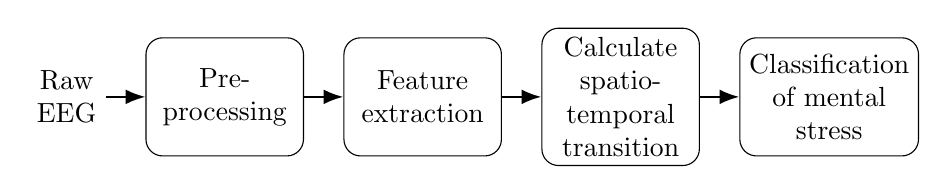
\begin{tikzpicture}[
        node distance=0.5cm,
        auto,
        block/.style={
            rectangle,
            draw,
            rounded corners=6pt, % Added rounding!
            minimum width=2cm,
            minimum height=1.5cm,
            text centered,
            align=center
            % Removed explicit fonts so it matches your document perfectly
        },
        plain/.style={
            text centered,
            align=center
        },
        line/.style={draw, -{Latex[length=2.5mm]}, thick}
    ]
        % Nodes
        \node [plain] (raw) {Raw\\EEG};
        \node [block, right=of raw] (pre) {Pre-\\processing};
        \node [block, right=of pre] (feat) {Feature\\extraction};
        \node [block, right=of feat] (calc) {Calculate\\spatio-\\temporal\\transition};
        \node [block, right=of calc] (class) {Classification\\of mental\\stress};

        % Paths
        \path [line] (raw) -- (pre);
        \path [line] (pre) -- (feat);
        \path [line] (feat) -- (calc);
        \path [line] (calc) -- (class);
    \end{tikzpicture}%
    }
    \caption{Analytical pipeline for the classification of mental stress.}
    \label{fig:eeg_pipeline}
\end{figure}

To extract meaningful data from an EEG signal, the data is processed in four steps~\cite[pg.~4]{ChatterjeeDebatri2023Doms}. First, a 30-second segment of data is pre-processed using a FIR band-pass filter to remove noise and an Automatic Artifact Removal tool suing Blind Source Separation-Canonical Correlation Analysis to remove extra signals from blinking or jaw clenching. Next, any important features are extracted and calculated. Hjorth parameters, which measure activity, mobility, and complexity, are calculated from the various frequencies of each 1-second chunk within the 30-second segment. Additionally, an Engagement Index is calculated as a ratio of beta band power to the sum of alpha and theta band power, which serves as a direct measurement of anxiety. Third, The spacio-temporal transition calculations map those features onto N x M matrices, where N is the number of EEG channels and M is the number of time windows. Those matrices are used to find maximum and minimum values for a feature, and track how they shift over time. Lastly, that data is classified into both binary stress levels (light vs. severe) and 4-class stress levels using a K-Nearest Neighbors. The study compared their classified binary and 4-level anxiety levels against the existing, state-of-the-art dataset, DASPS, and found that both binary and 4-level classifications were 83.8\% accurate~\cite[pg.~5]{ChatterjeeDebatri2023Doms}.

\subsection{Classifying Anxiety using a Convolutional Neural Network}
Three years later, a new paper examined using a Convolutional Neural Network (CNN) to further improve the accuracy of anxiety measurement in cheap EEG sensors, also comparing against the DASPS dataset~\cite{GhonchiHamidreza2025MMCA}. This paper theorized that deep learning models can better learn and model the complex patterns in EEG signals than traditional machine learning can. Additionally, deep learning can automatically extract relevant features, simplifying the path from raw data to anxiety classifications.

Using deep learning reduces the complexity in total calculations and additional data processing required. A CNN is trained on the raw EEG data, which learns and extracts the optimal frequency-based features~\cite{GhonchiHamidreza2025MMCA}. Those features are then fed into a Transformer, which adds weights to different parts of the signal, and uses the Squeeze-and-Excitation Attention method to evaluate the spacial relationships between different EEG channels on the scalp. Once fully trained, this pipeline also produces both binary and 4-level anxiety classifications, and achieves 82.94\% accuracy on binary and 74.05\% on 4-level. While the binary classification was able to match the DASPS' score of 83.5\%, the 4-level fell short, likely due to the dataset not being large enough to properly take advantage of deep learning's advantages.

\section{Application in Test-Taking Scenarios}
The above examined studies on axiety and EEG anxiety assessment provides a solid base to extrapolate how noise would effect anxiety while test-taking. White noise in the operating room showed no difference in anxiety level, while music decreased anxiety and auditory processing\cite{ShahrokhiShabnam2022Teow, WayT.JustinMD2013EoNo}. In an operating room, auditory processing is critical, but in an otherwise quiet test-taking environment, it is much less important so long as the ability to score well remains unaffected.

Listening to white noise shows no statistically significant reduction in anxiety or improvement in test scores, tested with a wearable EEG measuring anxiety. If there is a reduction in anxiety, there may also be an improvement in test scores. Additionally, we will test familiar and unfamiliar music, with the expectation that familair music reduces anxiety and improves test scores, while unfamiliar music reduces anxiety at the cost of lower test scores. Alternatively, familiar music may not improve test scores, or unfamilir music may improve test scores similarly to familiar music. Additionally, unfamiliar music can be split into distinct genres that may have varying levels of distraction: jazz, for example, may be less distracting than pop or rock music.

Using a wearable EEG that measures stress, we will test these claims by repeatedly taking tests while various kinds of noise play. EEGs have already proven to be accurate in tracking stress, and allows for continuous monitoring throughout test-taking~\cite{ChatterjeeDebatri2023Doms}. With an EEG, we can track how anxiety levels shift throughout the test-taking process, allowing for insights like when axiety is at its highest, and how much various kinds of noise dampen that peak. The EEG used will be a cheaper module, so one of the two anxiety classification methods examined above will be used. Without an excess of data to train on, the K-Nearest Neighbors algorithm is likely to yield more accurate nuanced results than the CNN algorithm would.

\section{Conclusion}
For a potential EEG wearable that measures stress while test-taking, various kinds of noise will change anxiety level and test performance. For example, music will likely reduce anxiety at the cost of lower test scores, while white noise may show little change~\cite{ShahrokhiShabnam2022Teow}. There are multiple existing methods of interpreting cheap EEG sensor data, which can compensate for the reduced signal accuracy and nearly match the DASPS benchmark dataset~\cite{ChatterjeeDebatri2023Doms, GhonchiHamidreza2025MMCA}. Of the two methods examined, the K-Nearest Neighbors algorithm produced more consistent data at the cost of additional computation and complexity, while the CNN produced worse results with lesser computations. For a prospective wearable measuring anxiety, either algorithm would be a solid choice, with the possibility of improving the CNN's results by manually collecting a large amount of data.

% ================
% 3. device design
% ================

To realize a wearable anxiety monitor, a NeuroSky MindWave Mobile 2 is being used. This headset was released in 2018, and included first-party software support on Windows, Android, and iOS~\cite{neurosky2018mwm2}. However, it appears that those pieces of software didn't receive significant updates post-release. Though the MindWave Mobile 2 is a relatively cheap electroencephalogram (EEG) headset, there are optimized algorithms that allow for accurate anxiety tracking, even on cheap EEGs~\cite{ChatterjeeDebatri2023Doms}.

For the physical wiring, the MindWave Mobile 2 only supports Bluetooth, with about equal software support on Windows and Android (the two OS's used by myself and Cameron). While direct sync to a PC or laptop using NeuroSky's software would likely work fine, I only have Linux installed on my laptop and desktop, potentially requiring a re-implementation of NeuroSky's software in a third-party program like OpenViBE~\cite{neurosky2018mwm2,openvibe2013}. However, both of us have Android phones, making NeuroSky's eegID mobile app a better option~\cite{neurosky2026eegid}. Setting up this app is relatively easy, requiring a manual connection in Bluetooth settings, then the app handles data recording and processing. To sync that data from the phone to a computer, it is easiest to export as a CSV file post-hoc. However, it would also likely be possible to stream the collected data in real-time or close to real-time using UDP or TCP (UDP is faster with fewer integrity checks on the data transmitted), though it may require a third-party app instead of eegID.

\begin{figure}[htbp]
    \centering
    % Forces the diagram to exactly 1 column width
    \resizebox{\columnwidth}{!}{%
    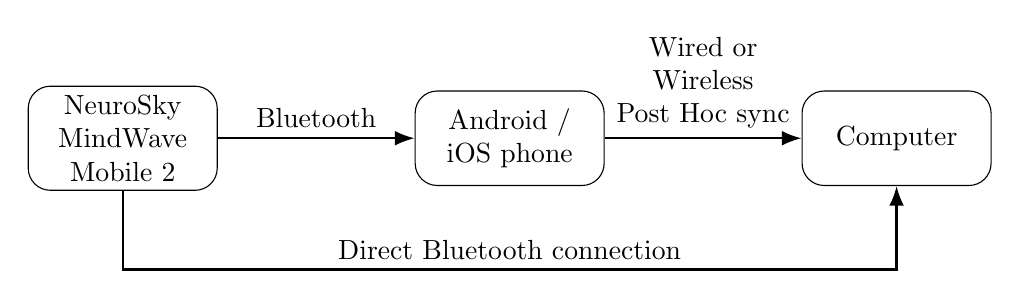
\begin{tikzpicture}[
        node distance=2.5cm, % Increased horizontal gap to prevent text overlap
        auto,
        block/.style={
            rectangle,
            draw,
            rounded corners=8pt, % Explicitly increased rounding
            minimum width=2.4cm,
            minimum height=1.2cm,
            text centered,
            align=center
            % Removed \bfseries so it perfectly inherits the IEEE standard text font
        },
        line/.style={draw, -{Latex[length=2.5mm]}, thick}
    ]
        % Nodes
        \node [block] (headset) {NeuroSky\\MindWave\\Mobile 2};
        \node [block, right=of headset] (phone) {Android /\\iOS phone};
        \node [block, right=of phone] (computer) {Computer};

        % Paths
        \path [line] (headset) -- node[align=center, above] {Bluetooth} (phone);
        
        % Broken into 3 lines to fit the gap perfectly
        \path [line] (phone) -- node[align=center, above] {Wired or\\Wireless\\Post Hoc sync} (computer);
        
        % Bottom path (Rerouted to tuck tightly under the blocks)
        \path [line] (headset.south) -- +(0,-1.0) -| node[near start, above, align=center] {Direct Bluetooth connection} (computer.south);
    \end{tikzpicture}%
    }
    \caption{Hardware data flow and synchronization architecture.}
    \label{fig:data_flow}
\end{figure}

% ===============
% 4. methods plan
% ===============

\section{Study Methods}
aExpanding upon last week's initial device design, much more detail on the specific methods is needed to properly focus this assignment. Previously, the tentative plan was to use a consumer wearable electroencephalogram (EEG) to measure anxiety levels during test-taking. The EEG selected is the NeuroSky MindWave Mobile 2, but the selection of test-taking proved a poor match for the scope of available participants for this study. With the main participants of any study conducted being myself and Cameron Brebner, it was not feasible to create an extended bank of test questions that would provide a difficult challenge and naturally induce anxiety. Instead, adapting the Trier Social Stress Test (TSST) to work between two people is much more achievable~\cite{kirschbaum_pirke_hellhammer_1993}. TSST traditionally was a way to induce anxiety in participants during an anticipation period and a test period though creating, then giving, a presentation of a random topic. However, at the end of the anticipation period (creating the presentation), the notes would be unexpectedly taken away, and the participant forced to give the 5-minute presentation blind. While this testing format works with fewer people, it can be adjusted and scaled to work with only two participants. Each of the two participants will create presentation notes and accompanying slides on something they are knowledgeable in, and the other participant will present on that topic to the first participant. Then, at a random time during the presentation, the notes will be taken away, and the presenter forced to finish the presentation using only what is on the slides themselves.

It is difficult to properly re-create TSST's anticipation period with a small number of participants, and no dedicated judges to add pressure onto the participants while creating presentations. Currently, this step does not induce anxiety aside from both participants knowing that they will need to trade presentations. However, it is difficult to induce anxiety without it being artificial, like playing stressful or unsettling music. However, taking EEG measurements during this phase can instead provide baseline brainwave readings while working in a low-stress environment. The slides would be created on a laptop which could be plugged into a projector or TV, while the notes written down on paper or printed out, making it easy to take them away later.

For the equivalent of TSST's test period, trading slide-decks and presenting blind mimics some of the induced stress from the original test. However, the participant giving the presentation will also be given the presentation notes at the beginning of the 5-minute presentation (5 minutes being chosen as an uncomfortable, but not completely unreasonable amount of time to present; also, because that is what TSST uses). This format loses TSST's surprise factor of the participant losing their notes at the beginning of the presentation, so it is added back in the form of taking away the presenting notes after a random amount of time. This reintroduces an unknown variable, even with prior knowledge, and creates two separate scenarios to measure anxiety under. While presenting with notes, it is stressful but possible thanks to said notes. After taking them away, the presenter is in a similar situation to the presenter from the TSST test, forced to present on something they are not comfortable with while not having notes.

If this study could be scaled up to a larger number of participants, it would be much more practical to use TSST as it was initially created, as the increased number of participants allows for it to run smoothly. However, this structure allows for a middle-ground to induce and measure anxiety with a small number of participants.

\section{Collecting Data}
During both phases, both participants will wear the EEG to record brain activity (for the preparation section, both participants can record brain activity by preparing slides and notes one at a time). The MindWave Mobile 2 records all of the data needed for anxiety analysis, as shown in Table~\ref{tab:eegid_brainwaves}. To record this data, the headset will be paired to a smartphone, and the data synced post-hoc to a laptop to perform data analysis. The chosen phone is a Motorola Moto X4, as it is about the same age as the headset and companion app, eegID~\cite{gsm_moto_x4_2017,neurosky2026eegid}. When attempting to install eegID on modern smartphones, there are significant issues with installing the older mobile app, and with reliably pairing the headset, which uses an older Bluetooth version. After recording brain activity through eegID, the CSV file is synced to an external computer for analysis, likely using KDE Connect to send the file to a paired computer~\cite{kde_connect_2026}.

All of the collected bands contain useful information on various components of anxiety. Notably, the Beta band can be subdivided into multiple categories associated with varying levels of anxiety, from none, slight, mild, moderate, and severe anxiety~\cite{ChatterjeeDebatri2023Doms}. Additionally, Theta waves are correlated with relaxation, and can become erratic while under stress~\cite{neurohealth_2019}. Gamma waves can also indicate agitation when the brain is over-aroused and highly anxious. Lastly, Alpha waves indicate a lack of anxiety, so unstable Alpha waves would indicate an anxiety response. There is a multitude of interesting literature on how to interpret specific bands of frequencies, and how to compare them to others, like Wei et al's study on how anxiety shapes theta band activity~\cite{wei_sun_long_2025}. However, adding much beyond a simple 4-level anxiety classification with some extra nuance and context from other brain activity would likely be beyond the scope of this study.

To apply these brainwave categorizations, relatively simple python scripting will suffice. Some of the more nuanced indicators, like disturbances in Alpha waves, may require comparing the variance in stressful and stress-free data, but the main classifications done will be relatively simple. The main hurdle will be accounting for error, from both the headset being cheap and possibly imprecise relative to medical-grade EEGs, and from the readings being taken through skin and bone. Chatterjee's study on training an AI on existing anxiety classifications from brain activity may prove a vital component while analyzing data, as the data may be somewhat unusable in the state it gets collected in~\cite{ChatterjeeDebatri2023Doms}.

\begin{table*}[t]
    \centering
    \caption{eegID Telemetry Fields and Correlated Brainwave States~\cite{neurosky2026eegid,neurohealth_2019}}
    \label{tab:eegid_brainwaves}
    \begin{tabularx}{\textwidth}{l l X}
        \hline
        \textbf{eegID Field} & \textbf{Frequency Range} & \textbf{Description and Meaning} \\
        \hline
        PoorSignal & N/A & A hardware metric indicating the quality of the sensor contact and signal integrity. \\
        EEG Raw Value & N/A & Unfiltered analog values captured directly from the EEG sensor. \\
        EEG Raw Value Volts & N/A & The raw EEG data scaled and converted into standard voltage units. \\
        Attention Level & N/A & A computed metric (ThinkGear algorithm) measuring the user's focus, concentration, and directed mental effort. \\
        Meditation Level & N/A & A computed metric (ThinkGear algorithm) measuring the user's level of mental calmness and relaxation. \\
        Blink Strength & N/A & A metric that detects eye blinks and quantifies their relative physical intensity. \\
        Delta & 1--3 Hz & Associated with deep, dreamless sleep, trance, and the unconscious mind. Represents a decreased awareness of the physical world. \\
        Theta & 4--7 Hz & Linked to intuition, creativity, daydreaming, internal focus, and spiritual awareness. Reflects the state between wakefulness and sleep. \\
        Alpha Low & 8--9 Hz & Correlates to an inner-awareness of self, mind/body integration, and balance. \\
        Alpha High & 10--12 Hz & Associated with centering, healing, and bridging the conscious to the subconscious. Promotes mental resourcefulness and calmness. \\
        Beta Low & 13--17 Hz & Reflects a state of being relaxed yet focused, integrated, and actively thinking while remaining aware of surroundings. \\
        Beta High & 18--30 Hz & Indicates high alertness and mental activity (e.g., math, planning), and general activation of mind/body functions, but can also reflect agitation. \\
        Gamma Low & 31--40 Hz & Consolidates information from different areas of the brain for simultaneous processing. Associated with alertness, good memory, or potential agitation. \\
        Gamma Mid & 41--50 Hz & Functions similarly to Gamma Low in consolidating rapid, simultaneous processing across brain regions; also indicates high alertness or agitation. \\
        \hline
    \end{tabularx}
\end{table*}

\bibliographystyle{IEEEtran}
\bibliography{references}

\end{document}
